\chapter{Traitement d'images}  

Un logiciel de traitement d'images est un logiciel qui permet d'effectuer des modifications sur une image existante : taille de l'image, luminosité, contraste, recadrage, etc...

{\footnotesize
\section*{Synoptique}
\begin{itemize}
\item Logiciel\footnote{Le logiciel \emph{Gimp} est librement téléchargeable : \url{http://www.gimp.org/}} : \emph{Gimp}
\item Matières concernées : français, SVT et arts visuels.
\item Compétences : 
        \begin{itemize}
        \item créer un chemin ;
	\item modifier un chemin existant ;
	\item tracer un trait le long d'un chemin ;
	\item écrire un texte le long d'un chemin ;
	\item utiliser les guides.
        \end{itemize}
\item Cette fiche est à réaliser :
        \begin{itemize}
	\item avant les vacances de février en SVT (séance 1) ;
        \item avant les vacances d'été en français (séance 2) ;
        \item avant la fin du semestre de cours en arts visuels (séance 3).
        \end{itemize}
\end{itemize}
}


\vspace{12pt}
%\section*{Les années précédentes, vous avez appris...}

Les compétences listées ci-dessous ont été vues en classes de 6\up{e} et de 5\up{e}. Vous en aurez à nouveau besoin pour les activités de cette année. Si nécessaire, reportez-vous aux \emph{Fiches MITIC} des années précédentes pour revoir comment :  

\begin{itemize}
\item exporter une image au format JPG ou PNG (6\up{e}) ;
\item recadrer une image avec l'outil de découpage (6\up{e}) ;
\item modifier la taille du canevas de l'image (6\up{e}) ;
\item régler la luminosité et le contraste de l'image (6\up{e}) ;
\item réaliser une capture d'écran (6\up{e} et 5\up{e}) ;
\item ajouter un texte et le mettre en forme (5\up{e}) ;
\item appliquer un filtre sur une portion de l'image (5\up{e}) ;
\item convertir une image en niveaux de gris (5\up{e}) ;
\item travailler avec les calques (5\up{e}). 
\end{itemize}




%\uneimageici{./images/texte03/Texte03_TableMatiere2}{.7\textwidth}%

%
%
%  S  É  A  N  C  E     I
%
%


%\pagebreak

\section{Séance 1 : Légender une image}\label{ficheImage4e2}

\subsection{Pour bien démarrer...}

Dès que vous avez ouvert un nouveau fichier dans \emph{Gimp}, sauvegardez-le suivant le format \texttt{Nom-seance1.png} (dans le menu \texttt{Fichier}, choisir \texttt{Enregistrer}). Pendant que vous travaillez, pensez à sauvegarder régulièrement votre travail (raccourci clavier \texttt{Cmd + s}).   

\uneimageici{./images/generales/clavierCmdS}{.4\textwidth}

%\vfill
%\phantom{rien}

\subsection{Sujet de l'activité...}

\vspace{10pt}

\boiteEnonceLarge{%
Le but de cette séance est d'ajouter des légendes à une image. Pour cela, vous devrez :
\begin{enumerate}
\item modifier si nécessaire la taille de l'image ; 
\item recadrer si nécessaire l'image à l'aide de l'outil de découpe ;
\item modifier si nécessaire la luminosité et le contraste de l'image afin de l'améliorer ; 
\item modifier la taille du canevas de l'image afin d'avoir de la place de côté pour placer les légendes ;
\item ajouter à l'aide de l'outil texte un titre à l'image ; 
\item positionner deux guides verticaux qui permettront d'aligner toutes les légendes (départ de flèches et début de texte) ;
\item pour chaque flèche de légende : créer un chemin, le tracer, puis écrire le texte associé au bout de la flèche.
\end{enumerate}

La figure ci-dessous montre l'image en cours de travail dans \emph{Gimp}. On remarque les guides (en bleu) utilisés pour l'alignement. Ici l'image a également été colorée sous \emph{Gimp} à l'aide de l'\emph{outil de remplissage} 
\includegraphics[width=.7cm]{./images/image03/iconePotPeinture}.
}

\boiteEnonceLarge{
\uneimageici{./images/image03/volcan/volcanEnCours}{.75\textwidth} 

Une fois votre travail terminé, exporter votre image au format PNG en la nommant à partir de votre nom : \texttt{Nom-seance1.png} puis rendre ce fichier sur Teams à l'endroit indiqué par votre enseignant (si nécessaire, se reporter à la fiche méthode \emph{Remettre son devoir}, page \pageref{TeamsRemettreDevoir}).
}% fin énoncé

\textbf{Pour obtenir de l'aide, rendez-vous à la page \pageref{Image4eOutils}}

\subsection{Pour aller plus loin...}

En informatique, les couleurs dérivent de trois couleurs maîtresses : le rouge, le vert et le bleu. Chercher sur Internet à quoi correspond l'instruction \texttt{rgb(255, 0, 0)}, et tester les différentes couleurs possibles à partir d'un \emph{color picker} tel que celui-ci : \\ \href{https://www.w3schools.com/colors/colors\_picker.asp}{https://www.w3schools.com/colors/colors\_picker.asp}.

\vfill

%\cadre{Pensez à sauver régulièrement votre travail en appuyant sur \texttt{Cmd + S} ou à partir du menu \texttt{Fichier} en choisissant \texttt{Enregistrer}.

%\uneimageici{./images/generales/clavierCmdS}{.5\textwidth}
%}



%
%  S  É  A  N  C  E     II
%
%


%\section{Séance 1 : un calligramme (français)}\label{ficheImage4e1}

%\boiteEnonceLarge{%
%Le but de cette séance est de réaliser un calligramme en écrivant un texte le long d'un chemin. Au départ, commencer par créer une nouvelle image de $600\times 600$ pixels. La figure ci-dessous montre un exemple obtenu en utilisant un chemin en forme d'arbre et en y inscrivant le début d'un poème de Jacques Prévert. Ici, l'image a été terminée en colorant le centre de l'arbre à l'aide de l'outil \emph{aérosol} puis recadrée.

%\uneimageici{./images/image03/calligramme/arbre}{.45\textwidth}

%Une fois votre travail terminé, exporter votre image au format PNG en la nommant à partir de votre nom : \texttt{Nom-Prénom-date.png} puis rendre ce fichier sur la plateforme \emph{Moodle} à l'endroit indiqué par votre enseignant (si nécessaire, se reporter à la fiche méthode \emph{Remettre un devoir sur Moodle}, section \vref{MoodleRendreDevoir}).
%} % fin énoncé

%\vfill

%\cadre{Pensez à sauver régulièrement votre travail en appuyant sur \texttt{Cmd + S} ou à partir du menu \texttt{Fichier} en choisissant \texttt{Enregistrer}.

%\uneimageici{./images/generales/clavierCmdS}{.5\textwidth}
%}


\newpage


\section{Séance 2 : Un calligramme}\label{ficheImage4e1}

%\vspace{-5em}

\subsection{Pour bien démarrer...}

Dès que vous avez ouvert un nouveau fichier dans \emph{Gimp}, sauvegardez-le suivant le format \texttt{Nom-seance2.png} (dans le menu \texttt{Fichier}, choisir \texttt{Enregistrer}). Pendant que vous travaillez, pensez à sauvegarder régulièrement votre travail (raccourci clavier \texttt{Cmd + s}).   

\uneimageici{./images/generales/clavierCmdS}{.4\textwidth}

\subsection{Sujet de l'activité...}

\vspace{10pt}

\boiteEnonceLarge{
Suivre pas à pas les instructions ci-dessous pour réaliser une image dans laquelle le texte suit un chemin tracé.

 %\texttt{arc-en-ciel.jpg}
\begin{enumerate}
\item Télécharger l'image \texttt{arbre.png} se trouvant sur la page Teams de votre cours.
\item Ouvrir cette image téléchargée avec le logiciel \emph{Gimp}.
\item Créer un chemin de gauche à droite en suivant la courbe de l'arbre et en commençant en bas à gauche (voir \S\ \vref{Gimp3cheminCreer}).
\item Sélectionner l'onglet \texttt{Calques}.
\item Écrire un texte le long du chemin (voir \S\ \vref{Gimp3cheminTexte}) avec l’outils \texttt{Texte} la phrase : \emph{\og La vie est comme un arc-en-ciel. Il faut de la pluie et du soleil pour en voir les couleurs. \fg}
\item Sélectionner le texte puis choisir la police de caractère \texttt{Colibri} et la taille 40. Choisir la couleur foncée de votre choix.
\item Faire un clic droit sur la phrase et choisir l'option \texttt{Texte le long du chemin}.
\item Créer un nouveau calque.
\setcounter{tmp}{\value{enumi}}  
\end{enumerate}
}

\vfill
\phantom{rien}

\boiteEnonceLarge{
\begin{enumerate}
\setcounter{enumi}{\value{tmp}}
\item Sélectionner ce nouveau calque et cliquer sur l'onglet \texttt{Chemins}.
\item  Dans l'onglet \texttt{Chemins} il y a maintenant deux chemins. Sélectionner celui du haut.
\item  Placer la flèche de la souris sur le chemin sélectionné et faire un clic droit dessus puis sélectionner l'option \texttt{Tracer un chemin}.
\item  Cliquer sur \texttt{Tracer} dans la fenêtre qui s'est ouverte.
\item  Revenir sur l’onglet \texttt{Calques}.
\item  Pour ne conserver que le texte tracé le long du chemin, cliquer sur l'œil qui est devant le calque contenant l'image de l'arc-en-ciel pour la faire disparaître ainsi que sur l'œil qui est devant le calque contenant le texte afin de le faire également disparaître.
\end{enumerate}

\uneimageici{./images/image03/calligramme/arbre.png}{.6\textwidth}

\item Une fois votre travail terminé, exporter votre image au format PNG (cliquer sur \texttt{Fichier} puis \texttt{Exporter sous}), et la nommer à partir de votre nom : \texttt{Nom-seance2.png} puis rendre ce fichier sur Teams à l'endroit indiqué par votre enseignant (si nécessaire, se reporter à la fiche méthode \emph{Remettre son devoir}, page \pageref{TeamsRemettreDevoir}).



%\vspace{-1em}
% ATTENTION J AI ENLEVE L IMAGE ET REMPLACE PAR ARBRE.PNG
%\deuximagesici{./images/image03/calligramme/arc-en-ciel}{.6\textwidth}%
    %{./images/image03/calligramme/resultat}{.6\textwidth}



%\vspace{-1em}


} % fin énoncé

\textbf{Pour obtenir de l'aide, rendez-vous à la page \pageref{Image4eOutils}}

%\vfill

%\cadre{Pensez à sauver régulièrement votre travail en appuyant sur \texttt{Cmd + S} ou à partir du menu \texttt{Fichier} en choisissant \texttt{Enregistrer}.

%\uneimageici{./images/generales/clavierCmdS}{.5\textwidth}
%}


\subsection{Pour aller plus loin...}

Utiliser un effet mirroir, pour afficher en-dessous de l'arbre que vous venez de construire un arbre symétrique par rapport au sol. Modifier également la couleur de ce second arbre.

%
%
%  S  É  A  N  C  E     III
%
%



\newpage

\section{Séance 3 : Composition d'une image}\label{ficheImage4e3}

\subsection{Pour bien démarrer...}

Dès que vous avez ouvert un nouveau fichier dans \emph{Gimp}, sauvegardez-le suivant le format \texttt{Nom-seance3.png} (dans le menu \texttt{Fichier}, choisir \texttt{Enregistrer}). Pendant que vous travaillez, pensez à sauvegarder régulièrement votre travail (raccourci clavier \texttt{Cmd + s}).   

\uneimageici{./images/generales/clavierCmdS}{.4\textwidth}

\subsection{Sujet de l'activité...}

\vspace{10pt}

\boiteEnonceLarge{%
Le but de cette séance est de composer une image à partir de deux images différentes choisies sur le site \emph{pexels.com}. Une première image est utilisée comme arrière-plan, sur lequel on ajoute un objet extrait par détourage d'une seconde image. Un exemple est montré ci-dessous : deux tigres issus d'une première image ont été «\,collés\,» sur une autre.

\uneimageici{./images/image03/tigreSalon/salonTigre}{.5\textwidth}


Une fois votre travail terminé, exporter votre image au format PNG en la nommant à partir de votre nom : \texttt{Nom-seance3.png} puis rendre ce fichier sur Teams à l'endroit indiqué par votre enseignant (si nécessaire, se reporter à la fiche méthode \emph{Remettre son devoir}, page \pageref{TeamsRemettreDevoir}).
}% fin énoncé

\textbf{Pour obtenir de l'aide, rendez-vous à la page \pageref{Image4eOutils}}



\subsection{Pour aller plus loin...}

Pour améliorer le rendu final, une \emph{ombre portée} peut être ajoutée (après avoir sélectionné le calque contenant l'objet extrait, dans le menu \texttt{Filtres} choisir \texttt{Ombres et Lumières} puis \texttt{Ombre en perspective}). Faire différents essais pour parvenir au résultat souhaité.




\vfill

%\cadre{Pensez à sauver régulièrement votre travail en appuyant sur \texttt{Cmd + S} ou à partir du menu \texttt{Fichier} en choisissant \texttt{Enregistrer}.

%\uneimageici{./images/generales/clavierCmdS}{.5\textwidth}
%}




% AIDE

\newpage

\section{Aide pour réaliser les activités}\label{Image4eOutils}
 
Les nouveaux outils dont vous aurez besoin pour réaliser les trois séances sur le traitement d'images sont décrits ci-dessous :

\begin{itemize}
\item créer et modifier un chemin, voir section \vref{Gimp3cheminCreer} ;
\item travailler avec les chemins et les calques, voir section \vref{Gimp3travaillerChemin} ; 
\item tracer un trait le long d'un chemin, voir section \vref{Gimp3cheminTracer} ;
\item écrire un texte le long d'un chemin, voir section \vref{Gimp3cheminTexte} ;
\item utiliser les guides, voir section \vref{Gimp3guide} ;
\item extraire un objet de son arrière plan (détourage), voir section \vref{Gimp3detourage}.
\end{itemize}  


\subsection{Créer et modifier un chemin}\index{Gimp!Créer un chemin}\index{Chemin : créer un chemin (Gimp)}\label{Gimp3cheminCreer} 

Un chemin est un ensemble de lignes (droites ou courbes) tracées entre des nœuds (ou \emph{«\,points d'ancrage\,»}). Le chemin n'est pas un élément graphique de l'image : c'est un guide qui permet de tracer des courbes sur l'image. Mais tant que le chemin n'est pas tracé (voir paragraphe \vref{Gimp3cheminTracer}), rien n'apparaît sur l'image. 

Pour créer un chemin, sélectionner l'outil \texttt{chemin} 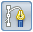
\includegraphics[width=1cm]{./images/image03/Chemin01} dans la palette d'outil.

Avec cet outil, chaque fois que l'on clique sur l'image, on ajoute un point d'ancrage du chemin (figure ci-dessous).

\uneimageici{./images/image03/Chemin02_1}{.3\textwidth}


On peut faire deux types de modifications sur un chemin existant, avec l'outil \texttt{chemin}: 
\begin{itemize}
\item Modifier la position des nœuds en cliquant et tirant dessus.
\item Courber les segments. Pour cela, cliquer sur un segment et tirer en gardant cliqué. Cette manipulation arrondit le segment et fait apparaître, de chaque côté du segment arrondi, deux autres segments terminés par des carrés. 

\uneimageici{./images/image03/Chemin02_2}{.3\textwidth}

En cliquant et tirant les carrés, on modifie l'arrondi de la courbe.
\uneimageici{./images/image03/Chemin02_3}{.3\textwidth}
\end{itemize}


\emph{Remarque :} quand un chemin est terminé, si on change d'outil, il «\,disparait\,» de l'écran. En fait le chemin a bien été créé. Pour le retrouver, il suffit de se rendre dans l'onglet \texttt{Chemins} (figure ci-dessous).

\uneimageici{./images/image03/Chemin03}{.3\textwidth}







\subsection{Travailler avec les chemins et les calques}\index{Gimp!Travailler avec les chemins et les calques}\index{Chemin : travailler avec les chemins et les calques (Gimp)}\label{Gimp3travaillerChemin}

Chemins et calques sont deux notions importantes dans les logiciels de traitement d'images. De le même manière que différents calques peuvent être créés, on peut créer différents chemins.

\subsubsection{Sélectionner le chemin sur lequel on travaille}\index{Gimp!Sélectionner le bon chemin}\index{Chemin : sélectionner le chemin sur lequel on travaille (Gimp)}

Si plusieurs chemins existent, il faut bien sélectionner celui avec lequel on veut travailler. Sur la figure ci-dessous, dans l'onglet chemin \circled{1}, on voit que trois chemins existent. Puisque c'est le \emph{chemin 2} qui est sélectionné \circled{2}, alors c'est lui qui peut être tracé ou c'est sur lui qu'un texte peut être écrit. On remarquera l'icône corbeille \circled{3} qui permet de supprimer un chemin existant.  

\uneimageici{./images/image03/CheminBoite}{.3\textwidth}


\subsubsection{Se placer sur le bon calque}\index{Gimp!Sélectionner le bon calque}\index{Calque : sélectionner le calque sur lequel on travaille (Gimp)}

Lorsqu'on veut tracer un chemin, il faut faire attention qu'un calque adapté soit sélectionné dans la fenêtre des calques. Ce n'est pas le cas sur la figure ci-dessous : dans l'onglet calque \circled{1} on voit que le calque contenant le \emph{Texte 2} \circled{2} est sélectionné. Et il est impossible de tracer quoi que ce soit dans un calque de texte. L'opération \emph{tracer un chemin} échouera. 

\uneimageici{./images/image03/CalqueBoite1}{.3\textwidth}

Le problème est corrigé sur la figure ci-dessous : un nouveau calque a été ajouté en cliquant sur l'icône \emph{Nouveau calque} \circled{1}. Le nouveau calque est bien sélectionné \circled{2} : l'opération \emph{tracer un chemin} peut avoir lieu.  

\uneimageici{./images/image03/CalqueBoite3}{.3\textwidth}





\subsection{Tracer un trait le long d'un chemin}\index{Gimp!Tracer un trait le long d'un chemin}\index{Chemin : tracer un trait le long d'un chemin (Gimp)}\label{Gimp3cheminTracer} 

Un chemin créé n'est pas encore un élément graphique de l'image. Pour qu'il soit tracé sur l'image, il faut : 

\begin{enumerate}
\item choisir la couleur dans laquelle le chemin doit être tracé ;
\item sélectionner l'onglet \texttt{chemin} et faire un clic droit sur le chemin que l'on veut tracer. Dans le menu qui s'ouvre, choisir \texttt{Tracer le chemin...} (il est également possible de passer par le menu \texttt{Édition} et de choisir \texttt{Tracer le chemin}) : 
\uneimageici{./images/image03/Chemin03}{.3\textwidth}
%\item dans la fenêtre qui s'ouvre, choisir \texttt{Tracer} et cliquer sur \texttt{Tracer le chemin}:
%\uneimageici{./images/image03/Chemin04}{.2\textwidth}
\item dans la boîte de dialogue qui apparaît, garder l'option \texttt{Ligne de tracé} et ajuster l'épaisseur du tracé avec \texttt{Épaisseur de ligne} :
\uneimageici{./images/image03/Chemin05}{.4\textwidth}
\item le chemin est alors tracé dans la couleur de premier plan sélectionnée. Supprimer la sélection du chemin (menu \texttt{Sélection}, choix \texttt{Aucune}) pour visualiser le tracé final:
\deuximagesici{./images/image03/Chemin06_1}{.6\textwidth}{./images/image03/Chemin06_2}{.65\textwidth}
\end{enumerate}

\subsection{Écrire un texte le long d'un chemin}\index{Gimp!Écrire un texte le long d'un chemin}\index{Texte le long d'un chemin (Gimp)}\label{Gimp3cheminTexte} 

\emph{Attention ! Le texte s'écrit le long du chemin en respectant l'ordre de création des différents nœuds du chemin. Il faut donc bien créer le chemin dans le même sens que celui souhaité pour le texte.}

\vspace{6pt}

Pour écrire un texte le long d'un chemin, procéder de la manière suivante : 

\begin{enumerate}
\item Tracer un chemin qui a la forme que l'on veut donner au texte et «\,l'arrondir\,». Par exemple :

\deuximagesici{./images/image03/TexteChemin01}{.5\textwidth}{./images/image03/TexteChemin02}{.5\textwidth}

\item Sélectionner l'\texttt{outil texte} 
\includegraphics[width=.6cm]{./images/image03/iconeTexte} dans la palette d'outils. Régler les paramètres pour le texte (police, taille, etc.) soit dans la boîte de dialogue \texttt{Texte} située en-dessous de la palette d'outil, soit en cliquant sur l'onglet paramètres (figures ci-dessous).

\deuximagesici{./images/image03/TexteChemin03}{.6\textwidth}{./images/image03/TexteChemin03bis}{.6\textwidth}

\item Écrire le texte souhaité. Si le texte est long, il peut être avantageux de faire un copier-coller depuis un logiciel de traitement de texte. 

\item Positionner le curseur de la souris sur le texte dans l'image, faire un clic droit et choisir l'option \texttt{Texte le long d'un chemin} (accessible uniquement si un chemin a déjà été créé). Le texte est alors positionné le long du chemin (attention, cette opération peut prendre un certain temps !). Il est également possible dans le menu \texttt{Calque} de choisir \texttt{Texte le long d'un chemin}. 
\deuximagesici{./images/image03/TexteChemin04}{.6\textwidth}{./images/image03/TexteChemin05}{.6\textwidth}

\emph{Il ne faut pas hésiter à annuler cette dernière étape (combinaison de touches \texttt{Cmd + Z}) si le résultat n'est pas celui attendu. Sélectionner alors à nouveau le texte pour en modifier la taille, la police ou le contenu puis placer le à nouveau le long du chemin. Recommencer encore et encore cette étape jusqu'à obtenir le résultat souhaité.}

\vspace{6pt}

\item Une fois satisfait du résultat obtenu, il faut tracer le chemin. La première étape consiste à se placer sur le calque où doit être tracé le chemin. Revenir ensuite sur l'onglet \texttt{Chemin}, effectuer un clic droit et choisir \texttt{Tracer le chemin}. Régler les différents paramètres puis terminer en cliquant sur le bouton \texttt{Tracer}. 

%\item En se positionnant dans la fenêtre des calques, on fait «\,disparaître\,» (l'affichage du chemin n'est plus actif) le texte initial et on se positionne sur le calque principal :
%\uneimageici{./images/image03/TexteChemin06bis}{.3\textwidth}

%\item Attention, le texte qui apparaît n'est qu'un chemin : il n'est pas encore un élément de l'image. Pour qu'il le devienne, il faut encore tracer le chemin : 

\deuximagesici{./images/image03/TexteChemin07}{.6\textwidth}{./images/image03/TexteChemin08}{.85\textwidth}

\uneimageici{./images/image03/TexteChemin09}{.5\textwidth}
\end{enumerate}

\subsection{Utiliser les guides}\index{Gimp!Utiliser les guides}\index{Guides (Gimp)}\label{Gimp3guide} 
Pour aider à la manipulation des images, tracer un chemin parfaitement horizontal, etc., on peut placer sur l'image des \emph{guides} horizontaux ou verticaux. Pour cela, cliquer dans la règle horizontale (exemple ci-dessous) ou la règle verticale qui encadrent la fenêtre de l'image et tirer un guide pour le positionner à l'endroit désiré.

\uneimageici{./images/image03/guides}{.5\textwidth}%

\emph{Remarque :} pour retirer un guide, sélectionner l'\texttt{outil de déplacement} 
\includegraphics[width=.6cm]{./images/image03/iconeDeplace}, cliquer sur le guide et le tirer en dehors de l'image. 

\subsection{Extraire un objet de son arrière plan (détourage)}\index{Gimp!Détourer une image}\index{Détourer une image (Gimp)}\index{Gimp!Extraire une image de son arrière plan}\index{Extraire une image de son arrière plan (Gimp)}\label{Gimp3detourage} 

L'objectif est de prélever un objet dans une image, par exemple ici une fleur que l'on veut copier sans son arrière plan. Cette opération d'extraction d'une partie de l'image se nomme \emph{détourage}. Le but est d'obtenir une sélection qui entoure parfaitement l'objet à prélever. On peut ainsi le copier et le coller dans une autre image, comme montré ci-dessous \emph{(source de l'image : pexels.com)}.

\deuximagesici{./images/image03/fleur}{.5\textwidth}{./images/image03/Detourage10}{.25\textwidth}


\textbf{Attention au choix de l'image !} Plus un objet est contrasté par rapport à l'arrière-plan de l'image, plus il sera facile à détourer. Il faut donc bien être vigilant au moment du choix de l'image contenant l'objet à extraire.

\vspace{6pt}

Pour détourer une image, on utilise l'outil \emph{extraction du premier-plan} disponible dans le menu \texttt{Outils}, \texttt{Outils de sélection} puis \texttt{Extraction du premier-plan} ou directement sur l'icône correspondante dans la boîte d'outils (voir ci-dessous).

\begin{enumerate}
\item Cliquer sur l'icône \emph{extraction du premier-plan} 
\includegraphics[width=.7cm]{./images/image03/iconeDetoure} : le pointeur de la souris prend la forme d'un lasso 
\includegraphics[width=.7cm]{./images/image03/iconeLasso}.
\item Sélectionner grossièrement l'objet à extraire en l'entourant (il faut sélectionner le moins possible d'arrière-plan afin de simplifier la suite du détourage) : il faut fermer la sélection en cliquant pour terminer sur le premier point créé.

\vspace{6pt}

\emph{Remarque :} faire des essais, utiliser la combinaison de touche \texttt{Cmd + Z} qui permet d'annuler la dernière action, recommencer et recommencer encore jusqu'à obtenir un résultat satisfaisant.

\vspace{6pt}

\item Dès qu'on ferme la sélection à l'aide du lasso, l'arrière-plan est recouvert d'un masque bleu et le pointeur de la souris change de forme : l'outil pinceau 
\includegraphics[width=.7cm]{./images/image03/iconePinceau} est sélectionné pour l'étape suivante. 
\uneimageici{./images/image03/Detourage02}{.3\textwidth}


\item Avec l'outil pinceau, tracer un trait continu à l'intérieur de l'objet à extraire de telle sorte que ce trait recouvre toutes les couleurs qui seront retenues pour l'extraction. Une technique simple consiste à peindre grossièrement tout l'objet à détourer.

\vspace{6pt}

Des zones n'ont pas été retenues (voir \circled{1} et \circled{2} sur l'image ci-dessous). Pour les zones à l'intérieur de l'objet à extraire \circled{1}, il est possible de tracer plusieurs traits au pinceau pour améliorer la sélection.

\deuximagesici{./images/image03/Detourage03}{.6\textwidth}{./images/image03/Detourage04}{.6\textwidth}

Pour la zone située à l'extérieur de l'objet à extraire \circled{2}, le traitement est effectué une fois l'objet extrait (voir plus bas).


\item Une fois satisfait du résultat, appuyer sur la touche \texttt{Entrée} pour terminer. L'objet à extraire est alors sélectionné (image à gauche ci-dessous). On peut alors copier puis coller l'objet dans une nouvelle image (image à droite ci-dessous). On voit que certaines zones (entourées en rouge) sont encore à éliminer.

\deuximagesici{./images/image03/Detourage05}{.5\textwidth}{./images/image03/Detourage06}{.45\textwidth}

\item Pour éliminer les dernières zones il faut utiliser les outils classiques de sélection, comme le lasso 
\includegraphics[width=.7cm]{./images/image03/outilLasso} (image de gauche ci-dessous), puis couper (\texttt{Cmd + X}) les zones sélectionnées (image au centre ci-dessous), ce qui permet d'éliminer la partie verte entre deux pétales (image à droite ci-dessous).

\vspace{6pt}

On peut également maintenir la touche \texttt{Shift} enfoncée pendant la sélection afin d'ajouter de nouvelles zones de l'image à la sélection courante. De même, la touche \texttt{Control} permet de retirer des parties de la sélection.

\troisimagesici{./images/image03/Detourage07}{.6\textwidth}{./images/image03/Detourage08}{.6\textwidth}{./images/image03/Detourage09}{.7\textwidth}

Petit à petit l'objet est «\,nettoyé\,» jusqu'au résultat voulu, comme montré ci-dessous.

\uneimageici{./images/image03/Detourage10}{.25\textwidth}

\end{enumerate}

\subsection{Aide pour la séance 3}

\subsubsection{Quelques conseils pour parvenir au résultat souhaité...}


\begin{minipage}[c]{.67\linewidth}
Lors du téléchargement des images sur le site \emph{pexels.com}, choisir une taille \emph{«\,Large\,»} qui est suffisante pour ce travail (figure ci-contre).

\vspace{6pt}

Les images doivent être choisies avec soin : choix de la situation, des couleurs, de l'objet à extraire, etc. Attention, l'objet à extraire doit être bien contrasté par rapport à son arrière-plan pour ne pas être trop difficile à détourer.

\end{minipage}\hfill
\begin{minipage}[c]{.27\linewidth}
\centering%
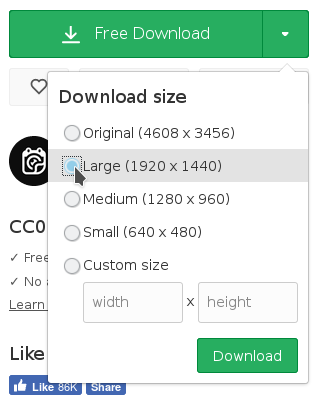
\includegraphics[angle=0,width=\textwidth]{./images/image03/pexelsDL}
\end{minipage}


Les deux images choisies pour réaliser l'exemple donné ici sont les suivantes :
 
\deuximagesici{./images/image03/tigreSalon/tigresIni}{\textwidth}{./images/image03/tigreSalon/salonIni}{\textwidth}







Une fois le détourage des tigres effectué (figure ci-dessous), la partie extraite est ajoutée à la seconde image à l'aide d'un copier-coller (on peut préalablement créer un nouveau calque transparent sur l'image contenant l'arrière-plan). 

\uneimageici{./images/image03/tigreSalon/tigres}{.15\textwidth}

Une fois le collage effectué, l'objet est redimensionné si nécessaire (après avoir sélectionné le calque contenant l'objet, dans le menu \texttt{Outils}, choisir \texttt{Outils de transformation} puis \texttt{Mise à l'échelle}, ou utiliser directement l'outil de mise à l'échelle 
\includegraphics[width=.7cm]{/images/image03/iconeMiseEchelle} disponible dans la palette d'outils). Les couleurs sont adaptées (réglage de la luminosité et du contraste ou encore de la teinte et de la saturation disponibles dans le menu \texttt{Couleurs}).



